

This section presents the core idea of our model generation and usage methodology.
%As mentioned earlier, our interest is to build a model that can capture the
%relationship between the resource utilization profiles and resultant CPU
%utilization when a pair of VMs transition from being dispersed to colocated,
%or vice versa.
We run a set of benchmarks, also referred to as micro-benchmarks, in both 
scenarios\textemdash{}dispersed and colocated\textemdash{}which exercise the utilization 
levels of VMs along different
axes\textemdash{}CPU, mutable and immutable network traffic, disk read and
write operations.


 \begin{table}
 \caption{Metrics considered per load type on each DomU (for predicting total CPU).}
%  \hspace{-0.2in}
 \begin{center}
 \begin{tabular}{|l|c|c|l|} \hline
  \bf{Disk} & \bf{Mutable} & \bf{Immutable} & \bf{CPU} \\ 
 & \bf{network} & \bf{network} & \\
  & \bf{traffic} & \bf{traffic} & \\ \hline
  Read (bytes/s) & Rx (Kbps) & Rx (Kbps) & User (\%) \\
  Write (bytes/s) & Tx (Kbps) & Tx (Kbps) & System (\%) \\
  Read (blocks/s) &  &  & Iowait (\%) \\
  Write (blocks/s) & &  & \\ \hline
 % Write blocks/sec & (NA) Tx Kbps & (A) Tx Kbps & System CPU\% \\
 %  &  &  & Iowait \\ \hline
 \end{tabular}
 \label{metrics-table}
 \end{center}
 \end{table}

\underline{Colocation and Dispersion models}: We wish to 
develop pair-wise CPU estimation models
that can predict total CPU requirement in target scenario
based on source scenario's resource usages.
Specifically, using resource usage measurements in the 
dispersed scenario, the ``colocation''
model predicts CPU utilization for the VM pair in the colocated scenario,
and based on the resource usage in the colocated deployments, while 
the ``dispersion''
model predicts the CPU utilization of VMs in the dispersed case.

Our benchmarking revealed that only the mutable network usage
causes change in CPU usage, upon change in VM placement.
Hence, we build models to use \underline{two approaches of prediction}:-
(i)~Predict \textit{total} CPU requirement based on multiple
resource usage profiles\textemdash{}CPU, disk and network,
(ii)~Predict \textit{differential} CPU requirement based only on
mutable network traffic metrics\textemdash{}later, take summation
of prediction with the source scenario's CPU usage to estimate
the total CPU requirement.
In this section, we explain both approaches in detail.

\subsection{Approach 1: Prediction of total CPU requirement}

\paragraph{Core Idea: } Using the profiling data from 
execution of micro-benchmarks and strengthened
by our conclusions in Section~\ref{sec:arescue-benchmark}, we 
believe that a generic linear model to estimate 
\textit{total} (dispersed or colocated) CPU resource usage
is realizable. 
The total CPU requirement of a virtual machine accounts for all its
activities, including usage of all other resources. Hence, the model
for predicting total CPU requirement has all resource metrics as its
parameters: (i)~$4$ metrics for mutable and
immutable transmit and receive network rates (in Kbps),
(ii)~$3$ CPU metrics of \texttt{iowait}, \texttt{system}
and \texttt{user} CPU (in \%), and
(iii)~$4$ metrics among disk read/write rates in
blocks/second and bytes/second. These metrics are
tabulated in Table~\ref{metrics-table}.
Since the correlation of all resource usages to CPU usage is linear, we employ
linear regression methods to build the models for CPU estimation.

\paragraph{Micro-benchmark Profiling: } The idea is to capture 
behaviour of resource usage in all possible conditions
for both dispersed and colocated scenarios. So, the micro-benchmarks
should span the full range of resource utilization levels. 
The workload micro-benchmarks are generated using the workload
generation procedures described previously (in 
Section~\ref{sec:arescue-setup}). 
For CPU micro-benchmarking, we split the CPU load on each VM
into $nine$ different intensities
ranging from $10\%$ to $90\%$. 
For network loads, we vary the load on each VM by steps 
of 10 Mbps, from 10 to 90 Mbps.
For disk read and write
micro-benchmarking, we vary the disk read/write rate from 
0 to 1280 blocks/second on each VM.

% Next, we describe briefly
% the approach adopted to ensure that we representatively
% cover the full range of resource utilization levels.

%For our profiling step, we use a generic client-server setup (described
%in more detail in Section~\ref{fig:setup}), wherein a \textit{client}
%(the controller machine) remotely connects to 
%the \textit{servers} (each PM or Dom0,
%and VM or DomU). % where workload is to be generated. 
%The workload generation
%tool resides on each such ``server'' and complies with the 
%load generation
%requests received from the ``client'' machine.
% 
% \textbf{SSS:Write up about micro-benchmarks. Also, mention
% the exponential number of cases to consider for combinational loads, and hence
% the randomized choice of combinational load cases.}

%clipped 10 feb
% \begin{itemize}
% \item \textbf{CPU micro-benchmark.}
% For CPU micro-benchmarking, we split the CPU load 
% into $nine$ different intensities
% ranging from $10\%$ to $90\%$. At each of the two VMs, 
% we vary the CPU load from $10\%$ to $90\%$, thus 
% resulting in $9 \times 9 = 81$ CPU workload
% combinations, as input for the modeling process.
% 
% \item \textbf{Network micro-benchmark.} 
% For network loads, we assume the maximum available capacity 
% to be $100Mbps$ and vary the load on each VM by steps 
% of $10Mbps$, from $10$ to $90 Mbps$.
% 
% \item \textbf{Disk read \& write micro-benchmarks.}
% For disk read and write
% micro-benchmarking, we vary the disk read/write rate from 
% 0 - 1280 blocks/second on each VM.
% For all files read and written, the block size is retained as $4 KB$.
% \end{itemize}


The set of inputs to train/build the models also includes 
combination workload benchmarks, which have CPU, network and disk
loads executed simultaneously, with different combinations of 
utilization levels.
However, to conduct exhaustive experiments that cover the
entire combination input set is not possible, since there is an
exponential number of cases in the input space of combinational load.
Thus, we adopted a workaround of choosing a set of random input 
workload types. 
For each combination benchmark, we sample a target utilization level, for 
each workload type, from a pre-defined range\textemdash{}CPU utilization from $10\%$ to 
$90\%$, network rate from 10 Mbps to 90 Mbps and disk read/write rate
of $0$ - $1280$ blocks/second. Each sample for a workload type is chosen
uniformly at random. 
This is intended to keep the sample points
uniformly distributed throughout the available sample space. 

Overall, for the model building, we used 956 sample points in total, consisting
of 200 points for CPU workload, 96 points for mutable network usage, 182 points
for immutable network usage, 162 points for disk read workload, 158 points for disk write 
workload and 158 combinational workloads.
% Thus, a combinational load input to a single VM would
% be a 6-tuple of the form,
% $<$\textit{c}$\%$, $a$ Mbps, $nrx$ Mbps, $ntx$ Mbps, $r$, \textit{w}$>$ \\ 
% where,
% $c$ is a random number in [1-100] for generating $c$\% CPU load,
% $a$ is a random number in [1-90] for generating $a~Mbps$ affine network
% receive traffic (correspondingly $a~Mbps$ transmit
% traffic at the other VM),
% $nrx$ is similarly random in [1-90] for generating non-affine network
% transmit traffic, 
% $ntx$ is random in [1-90] for generating non-affine network
% transmit traffic, 
% $r$ and $w$ are randomly chosen file read/write
% rates between 0 - 1280 blocks/second. Note that given a pair of VMs,
% the affine network traffic transmitted by one VM is the affine network
% traffic received by the other.



% \paragraph{Profiling Resource Usage:}
% We use the same setup as shown in Section~\ref{initial-benchmarking} (refer Fig.~\ref{f14})
% for the load generation and logging, described in this section. 

% \begin{table*}[t]
% \begin{center}
% \begin{tabular}{|l|l|l|l|} \hline
% Disk & Non-affine(NA) network & Affine(A) network & CPU \\ \hline
% Read req/sec & (NA) Rx Kbps & (A) Rx Kbps & CPU\% \\
% Write req/sec & (NA) Tx Kbps & (A) Tx Kbps & \\ \hline
% \end{tabular}
% \caption{Tabulation of metrics for black-box approach considered per load type on each DomU.}
% \label{blackbox-metrics-table}
% \end{center}
% \end{table*}

\paragraph{Multi-Linear Regression Modeling: }
Since the correlation of various resource usage metrics 
in the dispersed (colocated)
case to CPU utilization level in the colocated (dispersed) 
case emerged as approximately linear, we employ 
linear regression methods to build the models for CPU estimation.
Using values from the collected profiling data,
%a set of equations which represent the colocated CPU usage
the colocated CPU usage is represented as 
a linear function of the individually profiled resource metrics
in the corresponding dispersed scenario (i.e. dispersed scenario
stressed with the same workload),
and similarly dispersed CPU usage is represented as a linear function of 
the colocated resource usage metrics.
% Each such equation will be of the form as shown in Eqn. (\ref{mlr-eqn})
The relation between estimated CPU and resource parameters is shown
in Eqn. (\ref{mlr-eqn}).
\begin{equation}
\mbox{CPU}^{i}_{estimated} = C_{0} + C_{1} \times M^{i}_{1} + C_{2} \times M^{i}_{2} + ... + M^{i}_{m}
\label{mlr-eqn}
\end{equation}
where, $i$ is an iterator over each experiment or sample point
to be considered in the modeling, $m$ is
the number of parameters being considered, $M^{i}_{j}$ is
the value of parameter $M_{j}$ collected in the benchmark experiment number
$i$, and $\mbox{CPU}^{i}_{estimated}$ is the CPU usage 
either after dispersion or after colocation of VMs.
% The models that estimate the colocated CPU usage are referred 
% to as \textit{forward} models while 
% those that estimate the dispersed CPU utilization from the 
% colocated resource usage metrics are referred to as 
% \textit{reverse} models.
% In a \textit{forward} model, Dom0 %and DomU CPU usages
% CPU savings
% with colocated provisioning are predicted based on
% resource usages of VMs in the dispersed placements.
% In case of a
% black-box model (both forward and reverse), $m = 11$, and 
%The parameters considered per VM are, (i) $4$ metrics for mutable and 
%immutable transmit and receive network rates (in Kbps), 
%(ii) $3$ CPU metrics of \texttt{iowait}, \texttt{system} 
%and \texttt{user} CPU (in \%), and 
%(iii) $4$ metrics among disk read/write rates in 
%blocks/second and bytes/second. 
There are $11$ metrics in all to be considered, as discussed 
earlier in Table~\ref{metrics-table}. 
Both the colocation and dispersion DomU models have all these $11$ parameters.
The Dom0 \textit{colocation} model is built
with the metrics of both DomUs, and hence has $22$ parameters. 
The Dom0 \textit{dispersion} model 
depends on only one DomU's metrics at a time, and hence has only $11$
parameters.
% just like the DomU model. 
This is because the dispersed Dom0's CPU usage intuitively
depends on the resource usage of only its own hosted DomU and 
not on the other DomU of the VM pair.

\subsection{Approach 2: Prediction of differential CPU requirement}
\paragraph{Core idea: }
The difference in CPU usage upon transition between
colocated and dispersed placements of a VM pair, depends only on the mutable
network affinity between them. Hence, the idea here is to predict only
the difference, and sum it with the original scenario's CPU usage, to
obtain the total CPU requirement.
Note that differential Dom0 CPU is the difference in CPU 
usage between that incurred for the single (colocated) Dom0 and
the summation of both (dispersed) Dom0.
The model parameters are bit-rates (in Mbps) and packet-
rates (in packets per second) for both transmission (Tx) and reception (Rx), thus four parameters
in all: (i) Rx Mbps, (ii) Rx pkts/s, (iii) Tx Mbps, and (iv) Tx pkts/s. 

\paragraph{Modeling of differential CPU utilization: }
Since we predict only the difference in CPU usage, the total
CPU requirement of the migrating VM on the target can be computed
as the sum of the predicted value and the observed CPU usage on
the source PM. Formally, Eqn. (\ref{cpu-diff-eqn}) captures the
general notion of change in CPU usage ($\Delta\mbox{CPU}$)
while transitioning between colocated and dispersed scenarios.
\begin{equation}
	% \hspace{-0.3in}
	\Delta\mbox{CPU} = \mbox{CPU}^{scenario1} - \mbox{CPU}^{scenario2}
	\label{cpu-diff-eqn}
\end{equation}
where, scenario$\{1|2\}$ = $\{colocated|dispersed\}$.
In case of \textbf{Dom0's CPU usage}, colocated Dom0 CPU usage is incurred
for hosting both VMs whereas dispersed Dom0 usage levels are
on behalf of a single VM each. During transition from dispersed
(\textit{disp} for short) to colocated (\textit{colo} for short),
the change in Dom0 CPU is defined as the difference in CPU usage
between that incurred for the single (colocated) Dom0 and the
summation of both (dispersed) Dom0, as illustrated in
Eqn. (\ref{dom0-diff-eqn-fwd}).
%\hspace{-0.2in}
\begin{equation}
	% \hspace{-0.3in} \mbox{CPU}^{dom0}_{diff} = \mbox{CPU}^{{dom0}_{1}}_{dispersed} + \mbox{CPU}^{{dom0}_{2}}_{dispersed} - \mbox{CPU}^{dom0}_{colocated}
	% \hspace{-0.3in} 
	%\delta\mbox{Dom0CPU}^{colo} = \mbox{Dom0CPU}^{colo} - \displaystyle\sum\limits_{i=1,2}\mbox{Dom0CPU}^{disp}
	\Delta\mbox{CPU}^{colo}_{Dom0} = \mbox{CPU}^{colo}_{Dom0} - \displaystyle\sum\limits_{i=1,2}\mbox{CPU}^{disp}_{Dom0}
	\label{dom0-diff-eqn-fwd}
\end{equation}
Similarly, during transition from colocated to dispersed, change in
CPU usage for each Dom0 instance is,
\begin{equation}
	% \hspace{-0.2in} 
	\Delta\mbox{CPU}^{disp}_{Dom0} = \mbox{CPU}^{disp}_{Dom0} - \frac{\mbox{CPU}^{colo}_{Dom0}}{2} %\frac{{CPU}^{dom0}_{colocated}}{2} 
	\label{dom0-diff-eqn-rev}
\end{equation}
% where i = 1,2.
Here we use %$\frac{{CPU}^{dom0}_{colocated}}{2}$ 
$\mbox{CPU}^{colo}_{Dom0}$/2
% as an approximation of CPU usage incurred
% for a single VM within the colocated scenario. Intuitively, the Dom0
% CPU usage incurred per VM in a colocated setting is different than
% that incurred in a dispersed setting, when intra-PM traffic is involved.
% This is % in Eqn. (\ref{dom0-diff-eqn-rev}) 
since colocated Dom0 CPU usage
is incurred on behalf of both VMs whereas we wish to predict
dispersed Dom0 CPU usage incurred on behalf of only a single VM each.
So, we use $\mbox{CPU}^{colo}_{Dom0}$/2 as an approximation of CPU usage
incurred for a single VM within the colocated scenario.
% so that the difference between Dom0
% usage on behalf of each VM in colocated and dispersed cases can be computed.
In case of \textbf{DomU's CPU usage}, we define change
in CPU as shown in Eqn. (\ref{domu-diff-eqn}).
\begin{equation}
	\Delta\mbox{CPU}_{DomU} = \mbox{CPU}^{disp}_{DomU} - \mbox{CPU}^{colo}_{DomU}
	\label{domu-diff-eqn}
\end{equation}
Based on Eqn. (\ref{domu-diff-eqn}), the difference needs to
be added to or subtracted from the observed CPU usage depending upon
whether the VM's migration results in dispersion or colocation, respectively. 
Thus, DomU's
colocation and dispersion models are one and the same, since the
\textit{magnitude} of the difference in CPU usage is the same in both
directions.

Using values from the collected profiling data,
%a set of equations which represent the colocated CPU usage
difference in CPU usage is represented as a linear function of the
individually profiled network usage metrics in dispersed
scenario (i.e. dispersed scenario stressed with the same workload).
The relation between estimated CPU and resource parameters is the
same as shown earlier in Eqn.~\ref{mlr-eqn}, except that
the value being estimated is the difference in CPU usage
and not the total.
In the case of DomU model, the CPU usage estimate is expectedly a
function of its own network usage rates and uses all these four
metrics in its model. Similarly, in the case of Dom0 colocation model,
colocated Dom0 CPU usage accounts for both the colocated DomUs
and hence should intuitively depend on four metrics each of
both the DomUs, i.e. eight metrics in total. However, given a VM pair
with only mutual network communication, the received traffic by one
VM is the transmitted
traffic by the other, hence the metrics of one VM are in fact
duplicates of the metrics of the other, albeit in a different
order. We discard the redundant columns, therefore even Dom0
model has only four parameters. Thus, each model can be represented as
\begin{equation}
	% \mbox{CPU}_{est} = C_{0} + C_{1} \times Aff^{Rx}_{MBps} + C_{2} \times Aff^{Tx}_{MBps} + Aff^{Rx}_{pps} + Aff^{Tx}_{pps}
	% \hspace{-0.3in} \mbox{CPU}_{est} = C_{0} + C_{1} Aff^{R}_{K} + C_{2} Aff^{T}_{K} + C_{3} Aff^{R}_{P} + C_{4} Aff^{T}_{P}
	%\begin{split}
	\hspace{-0.3in} \Delta\mbox{CPU}_{est} = C_{0} + C_{1} \mbox{MutRx}_{Kbps} + C_{2} \mbox{MutRx}_{p/s} \\ 
	+ C_{3} \mbox{MutTx}_{Kbps}  + C_{4} \mbox{MutTx}_{p/s}
	%\end{split}
	\label{mlr-eqn-2}
\end{equation}
 where, ``Mut'' stands for mutable network traffic,
  superscripts Rx \& Tx stands for receive \& transmit, and
  subscripts Kbps \& p/s represent the units Kbps and packets/second,
  respectively.
\\
\\
To solve for the $m+1$ coefficients $C_{k}$, a stepwise linear
regression approach can help to select the ``best'' set of parameters.
%, in a stepwise manner.
% that would result in the most optimal prediction for the given learning dataset. 
% Thus, a model is learnt based only on these selected set of metrics. 
The stepwise approach ensures that only significant parameters that influence 
the predicted value are part of the model~\cite{applied-regression-analysis}.
For our implementation, we use the
% LARS~\cite{lars} package %present in Python~\cite{python} 
Robustbase package~\cite{robustbase}, part of the R statistical computing
environment, for robust and stepwise linear regression.
The linear regression solver, takes as input $M^{i}_{j}$ values for the 
various workloads and outputs values of $C_{k}$ that 
best predict CPU utilization. The set of coefficients thus
derived is the model that describes the relation between the $k$ parameters
and the total or differential CPU usage.

\subsection{Applying the pair-wise models to multi-VM scenarios}
\label{sec:multi-vm}
In order to apply the pair-wise models to situations with multiple
VMs hosting different applications
that may have different number of communicating tiers, the
first step needed is to consider that in a multi-VM scenario,
a single VM migration step
can result in not only dispersion w.r.t one (or a few) VM(s), but
also in colocation w.r.t other VM(s).
%To be more specific, the models that we have constructed so far
%apply to a single pair of VMs at a time i.e., in a single VM
%migration step, either two dispersed
%VMs can get colocated or two colocated VMs can get dispersed.
%In order to apply this CPU usage model to a real multi-VM 
%scenario, we need to be able to predict the CPU utilization 
%even in a combined scenario, wherein 
Fig.~\ref{fig:forward-plus-reverse} illustrates the case where
a single VM is being dispersed from one VM and colocated with another.
%Note that the terms DomU and VM are used interchangeably
%in this description and figure. 
Suppose $VM1$, $VM2$ and $VM3$ host different tiers of a 3-tier application.
As can be seen, one VM migration can result in that VM ($VM2$ in
Fig.~\ref{fig:forward-plus-reverse}) being dispersed from one VM ($VM1$)
on the source PM and being colocated with another VM ($VM3$) on
the target PM.

%Further, a VM that is communicating with multiple
%colocated VMs would get dispersed from all of them due to a single
%migration step. 
In the general multi-VM scenario, any particular VM (say $VM_{x}$)
may have multiple communicating neighbors, each of them belonging to
exactly one of three sets, (i) \textit{affinity-at-source}
(ii) \textit{affinity-at-target}, and (iii) \textit{affinity-at-other}.
Migration of $VM_{x}$ will cause it to become dispersed from
its \textit{affinity-at-source} set and colocated with its
\textit{affinity-at-target} set.
We refer to this dual step of being dispersed from
\textit{affinity-at-source} set and being colocated with
\textit{affinity-at-target} set, as a \textit{combined transition}.
In this case, the CPU utilization of all VMs in the
\textit{affinity-at-source} \& \textit{affinity-at-target} sets and
the migrating VM itself are expected to change.
In fact, the \textit{colocation}
and the \textit{dispersion} transitions can be viewed as
special cases of the \textit{combined} transition, starring only 
two VMs, with the dispersion transition being the case where 
dispersion set on source PM is empty while the dispersion transition 
is the case with an empty set on target PM.
Our aim is to predict the resource usage of all affected VMs and PMs.

\begin{figure}[t]
	\centering
	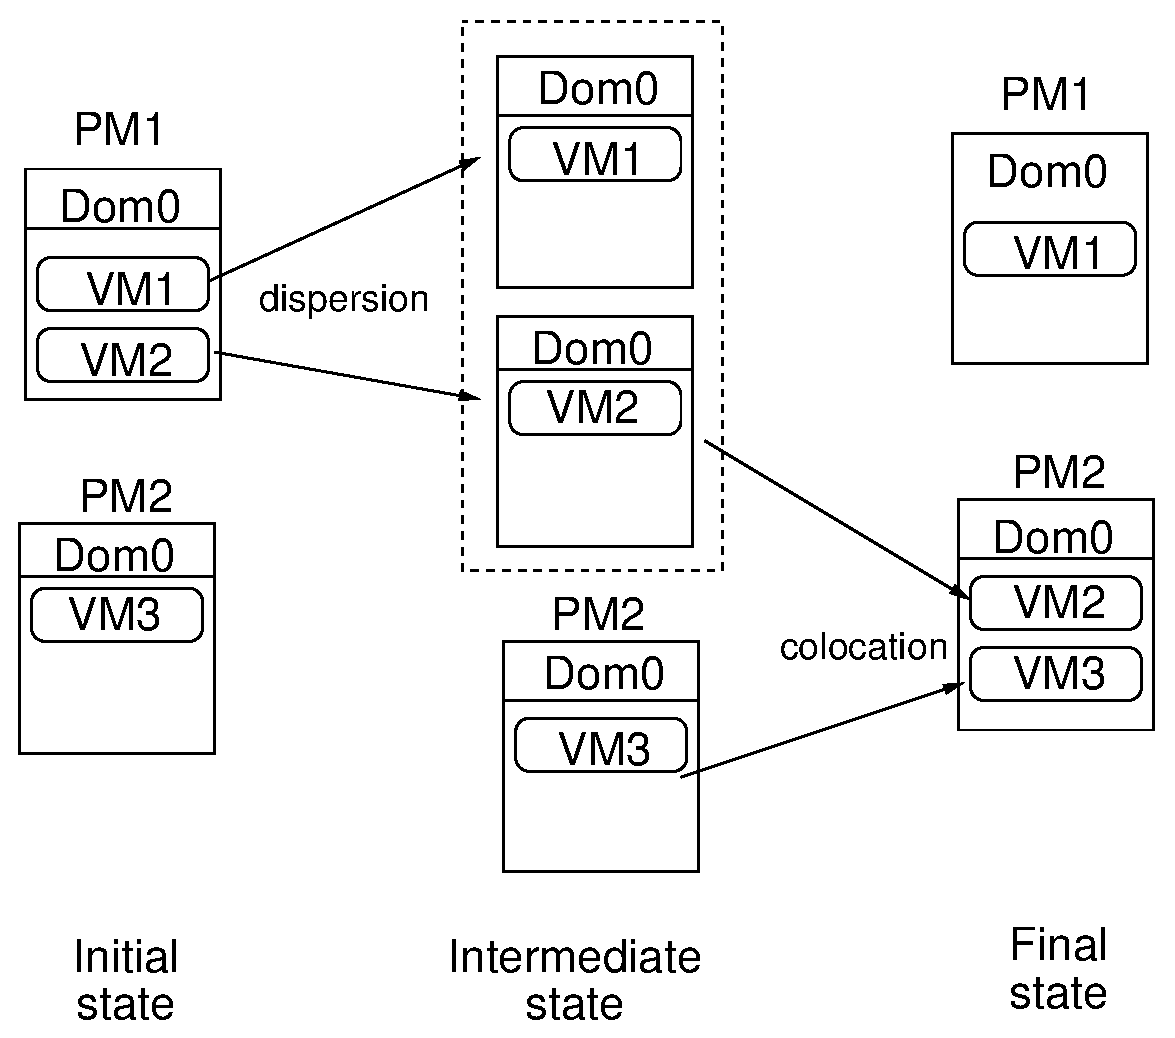
\includegraphics[scale=0.45]{jss-figures/new-forward-plus-rev.eps}
	\caption{Combined transition for $VM2$}
	\label{fig:forward-plus-reverse}
\end{figure}
% Our aim is to predict the CPU utilization when $VM2$'s migration
% causes a change in placement from \textit{Configuration1} to \textit{Configuration2}
% or vice versa. 

Consider the combined transition illustrated in Fig.~\ref{fig:forward-plus-reverse}.
It is straight-forward
to apply the DomU \textit{colocation} and \textit{dispersion} models to
$VM1$ and $VM3$ to predict their resultant CPU usages. Similarly, $PM1$'s
Dom0 CPU usage can also be predicted by applying Dom0 dispersion model.
However, prediction of $VM2$'s and $PM2$'s resultant CPU usage after this
combined transition needs a multi-phase prediction methodology.
The basic idea is to first apply the \textit{dispersion model} to the
measured metrics corresponding to network-affinity level between $VM2$
to/fro the \textit{affinity-at-source} set, and then use this
intermediate estimate
%This is an intermediate estimate and is used 
to make final prediction based upon network-affinity level
between $VM2$ to/fro the \textit{affinity-at-target} set. Intuitively,
VMs in the \textit{affinity-at-other} set do not affect CPU
requirement of the migrating $VM2$ because the nature of network-affinity
between them stays the same (\textit{immutable}) both before and
after migration.
\\
\\
In this section, we described our model-building process and described
the synthetic training datasets used to learn this model.
We also described the process of applying the pair-wise prediction
models to multi-VM scenarios.
Though the models are built with synthetic data-sets in which
TCP data-rates are generated by manipulating the application level
segment size and the periodicity of transmission, the application
scenarios for the models are not expected to have such controlled
behaviour. In particular, though the applications are
expected to use TCP for communication, the application-level
segment sizes and the inter-request times (also called think-times)
would be significantly more random. In the next section, we experimentally
evaluate the models on randomized synthetic data as well as on
benchmark application data. We also apply the model to multi-VM
scenarios and evaluate prediction effectiveness.
